% Options for packages loaded elsewhere
\PassOptionsToPackage{unicode}{hyperref}
\PassOptionsToPackage{hyphens}{url}
%
\documentclass[
]{article}
\usepackage{amsmath,amssymb}
\usepackage{lmodern}
\usepackage{iftex}
\ifPDFTeX
  \usepackage[T1]{fontenc}
  \usepackage[utf8]{inputenc}
  \usepackage{textcomp} % provide euro and other symbols
\else % if luatex or xetex
  \usepackage{unicode-math}
  \defaultfontfeatures{Scale=MatchLowercase}
  \defaultfontfeatures[\rmfamily]{Ligatures=TeX,Scale=1}
\fi
% Use upquote if available, for straight quotes in verbatim environments
\IfFileExists{upquote.sty}{\usepackage{upquote}}{}
\IfFileExists{microtype.sty}{% use microtype if available
  \usepackage[]{microtype}
  \UseMicrotypeSet[protrusion]{basicmath} % disable protrusion for tt fonts
}{}
\makeatletter
\@ifundefined{KOMAClassName}{% if non-KOMA class
  \IfFileExists{parskip.sty}{%
    \usepackage{parskip}
  }{% else
    \setlength{\parindent}{0pt}
    \setlength{\parskip}{6pt plus 2pt minus 1pt}}
}{% if KOMA class
  \KOMAoptions{parskip=half}}
\makeatother
\usepackage{xcolor}
\usepackage[margin=1in]{geometry}
\usepackage{color}
\usepackage{fancyvrb}
\newcommand{\VerbBar}{|}
\newcommand{\VERB}{\Verb[commandchars=\\\{\}]}
\DefineVerbatimEnvironment{Highlighting}{Verbatim}{commandchars=\\\{\}}
% Add ',fontsize=\small' for more characters per line
\usepackage{framed}
\definecolor{shadecolor}{RGB}{248,248,248}
\newenvironment{Shaded}{\begin{snugshade}}{\end{snugshade}}
\newcommand{\AlertTok}[1]{\textcolor[rgb]{0.94,0.16,0.16}{#1}}
\newcommand{\AnnotationTok}[1]{\textcolor[rgb]{0.56,0.35,0.01}{\textbf{\textit{#1}}}}
\newcommand{\AttributeTok}[1]{\textcolor[rgb]{0.77,0.63,0.00}{#1}}
\newcommand{\BaseNTok}[1]{\textcolor[rgb]{0.00,0.00,0.81}{#1}}
\newcommand{\BuiltInTok}[1]{#1}
\newcommand{\CharTok}[1]{\textcolor[rgb]{0.31,0.60,0.02}{#1}}
\newcommand{\CommentTok}[1]{\textcolor[rgb]{0.56,0.35,0.01}{\textit{#1}}}
\newcommand{\CommentVarTok}[1]{\textcolor[rgb]{0.56,0.35,0.01}{\textbf{\textit{#1}}}}
\newcommand{\ConstantTok}[1]{\textcolor[rgb]{0.00,0.00,0.00}{#1}}
\newcommand{\ControlFlowTok}[1]{\textcolor[rgb]{0.13,0.29,0.53}{\textbf{#1}}}
\newcommand{\DataTypeTok}[1]{\textcolor[rgb]{0.13,0.29,0.53}{#1}}
\newcommand{\DecValTok}[1]{\textcolor[rgb]{0.00,0.00,0.81}{#1}}
\newcommand{\DocumentationTok}[1]{\textcolor[rgb]{0.56,0.35,0.01}{\textbf{\textit{#1}}}}
\newcommand{\ErrorTok}[1]{\textcolor[rgb]{0.64,0.00,0.00}{\textbf{#1}}}
\newcommand{\ExtensionTok}[1]{#1}
\newcommand{\FloatTok}[1]{\textcolor[rgb]{0.00,0.00,0.81}{#1}}
\newcommand{\FunctionTok}[1]{\textcolor[rgb]{0.00,0.00,0.00}{#1}}
\newcommand{\ImportTok}[1]{#1}
\newcommand{\InformationTok}[1]{\textcolor[rgb]{0.56,0.35,0.01}{\textbf{\textit{#1}}}}
\newcommand{\KeywordTok}[1]{\textcolor[rgb]{0.13,0.29,0.53}{\textbf{#1}}}
\newcommand{\NormalTok}[1]{#1}
\newcommand{\OperatorTok}[1]{\textcolor[rgb]{0.81,0.36,0.00}{\textbf{#1}}}
\newcommand{\OtherTok}[1]{\textcolor[rgb]{0.56,0.35,0.01}{#1}}
\newcommand{\PreprocessorTok}[1]{\textcolor[rgb]{0.56,0.35,0.01}{\textit{#1}}}
\newcommand{\RegionMarkerTok}[1]{#1}
\newcommand{\SpecialCharTok}[1]{\textcolor[rgb]{0.00,0.00,0.00}{#1}}
\newcommand{\SpecialStringTok}[1]{\textcolor[rgb]{0.31,0.60,0.02}{#1}}
\newcommand{\StringTok}[1]{\textcolor[rgb]{0.31,0.60,0.02}{#1}}
\newcommand{\VariableTok}[1]{\textcolor[rgb]{0.00,0.00,0.00}{#1}}
\newcommand{\VerbatimStringTok}[1]{\textcolor[rgb]{0.31,0.60,0.02}{#1}}
\newcommand{\WarningTok}[1]{\textcolor[rgb]{0.56,0.35,0.01}{\textbf{\textit{#1}}}}
\usepackage{longtable,booktabs,array}
\usepackage{calc} % for calculating minipage widths
% Correct order of tables after \paragraph or \subparagraph
\usepackage{etoolbox}
\makeatletter
\patchcmd\longtable{\par}{\if@noskipsec\mbox{}\fi\par}{}{}
\makeatother
% Allow footnotes in longtable head/foot
\IfFileExists{footnotehyper.sty}{\usepackage{footnotehyper}}{\usepackage{footnote}}
\makesavenoteenv{longtable}
\usepackage{graphicx}
\makeatletter
\def\maxwidth{\ifdim\Gin@nat@width>\linewidth\linewidth\else\Gin@nat@width\fi}
\def\maxheight{\ifdim\Gin@nat@height>\textheight\textheight\else\Gin@nat@height\fi}
\makeatother
% Scale images if necessary, so that they will not overflow the page
% margins by default, and it is still possible to overwrite the defaults
% using explicit options in \includegraphics[width, height, ...]{}
\setkeys{Gin}{width=\maxwidth,height=\maxheight,keepaspectratio}
% Set default figure placement to htbp
\makeatletter
\def\fps@figure{htbp}
\makeatother
\setlength{\emergencystretch}{3em} % prevent overfull lines
\providecommand{\tightlist}{%
  \setlength{\itemsep}{0pt}\setlength{\parskip}{0pt}}
\setcounter{secnumdepth}{-\maxdimen} % remove section numbering
\usepackage{booktabs}
\usepackage{longtable}
\usepackage{array}
\usepackage{multirow}
\usepackage{wrapfig}
\usepackage{float}
\usepackage{colortbl}
\usepackage{pdflscape}
\usepackage{tabu}
\usepackage{threeparttable}
\usepackage{threeparttablex}
\usepackage[normalem]{ulem}
\usepackage{makecell}
\usepackage{xcolor}
\ifLuaTeX
  \usepackage{selnolig}  % disable illegal ligatures
\fi
\IfFileExists{bookmark.sty}{\usepackage{bookmark}}{\usepackage{hyperref}}
\IfFileExists{xurl.sty}{\usepackage{xurl}}{} % add URL line breaks if available
\urlstyle{same} % disable monospaced font for URLs
\hypersetup{
  pdftitle={USAGE},
  pdfauthor={Boniface Kalong},
  hidelinks,
  pdfcreator={LaTeX via pandoc}}

\title{USAGE}
\author{Boniface Kalong}
\date{2023-05-15}

\begin{document}
\maketitle

\begin{Shaded}
\begin{Highlighting}[]
\FunctionTok{library}\NormalTok{(readxl)}
\NormalTok{USAGE }\OtherTok{\textless{}{-}} \FunctionTok{read\_excel}\NormalTok{(}\StringTok{"USAGE.xlsx"}\NormalTok{)}
\end{Highlighting}
\end{Shaded}

\begin{verbatim}
## New names:
## * `` -> `...13`
\end{verbatim}

\begin{Shaded}
\begin{Highlighting}[]
\NormalTok{USAGE\_xlsx }\OtherTok{=}\NormalTok{ USAGE}
\FunctionTok{colnames}\NormalTok{(USAGE\_xlsx)}
\end{Highlighting}
\end{Shaded}

\begin{verbatim}
##  [1] "Timestamp"                                                                                                        
##  [2] "Please indicate your gender"                                                                                      
##  [3] "Highest level of education"                                                                                       
##  [4] "Where are you employed?"                                                                                          
##  [5] "What is your age range?"                                                                                          
##  [6] "How long have you been a subscriber to the National Health Insurance Scheme"                                      
##  [7] "Have you accessed healthcare under the National Health Insurance Scheme before?"                                  
##  [8] "How do you see healthcare delivery under the National Health Insurance Scheme?"                                   
##  [9] "Do you know about the NHIS Mobile Renewal Service?"                                                               
## [10] "Have you ever used the Mobile Renewal Service before?"                                                            
## [11] "If yes, how will you rate the service?"                                                                           
## [12] "Do you agree that the Mobile Renewal Service should be continued or suspended"                                    
## [13] "...13"                                                                                                            
## [14] "Using the Mobile Renewal Service enables me to renew my health insurance faster."                                 
## [15] "The Mobile Renewal Service saves me time and resources in renewing my health insurance"                           
## [16] "The Mobile Renewal Service enhances my effectiveness in renewing my health insurance"                             
## [17] "The Mobile Renewal Service increases productivity in healthcare delivery"                                         
## [18] "The Mobile Renewal Service is easy to use"                                                                        
## [19] "Learning to use the Mobile Renewal Service is easy"                                                               
## [20] "Interactions with the System requires a lot of mental effort."                                                    
## [21] "My interactions with the system is clear and understandable"                                                      
## [22] "i will use the Mobile Renewal Service to renew my health insurance"                                               
## [23] "I am aware of the benefits of using the Mobile Renewal Service as much as possible"                               
## [24] "If I have access to mobile money services, I will use the Mobile Renewal Service"                                 
## [25] "Mobile Renewal Service offers useful and satisfying services"                                                     
## [26] "The quality of Mobile Renewal Service is good"                                                                    
## [27] "The use of Mobile Renewal Service has a high cost"                                                                
## [28] "The service charge by the telecommunication companies for using the Mobile Renewal Service is high"               
## [29] "I face some financial barriers to use the Mobile Renewal Service"                                                 
## [30] "The Mobile Renewal Service is always accessible"                                                                  
## [31] "Disruptions and problems always occur in accessing the Mobile Renewal Service"                                    
## [32] "Mobile Renewal Service is available everywhere and every time even on holidays."                                  
## [33] "The Mobile Renewal Service is reliable"                                                                           
## [34] "The Mobile Renewal Service is authentic and reliable in its claims"                                               
## [35] "I trust the telecommunication operators to provide secure data communication for using the Mobile Renewal Service"
## [36] "The use of the Mobile Renewal Service will not disclose my personal information"                                  
## [37] "I am satisfied with the overall performance of the Mobile Renewal Service"
\end{verbatim}

\begin{Shaded}
\begin{Highlighting}[]
\FunctionTok{library}\NormalTok{(DataExplorer)}
\FunctionTok{introduce}\NormalTok{(USAGE)}
\end{Highlighting}
\end{Shaded}

\begin{verbatim}
## # A tibble: 1 x 9
##    rows columns discrete_columns continuous_columns all_missing_columns
##   <int>   <int>            <int>              <int>               <int>
## 1   418      37               13                 24                   0
## # i 4 more variables: total_missing_values <int>, complete_rows <int>,
## #   total_observations <int>, memory_usage <dbl>
\end{verbatim}

\begin{Shaded}
\begin{Highlighting}[]
\FunctionTok{plot\_intro}\NormalTok{(USAGE)}
\end{Highlighting}
\end{Shaded}

\includegraphics{USAGE_files/figure-latex/unnamed-chunk-3-1.pdf}

Function to abbreviate columns by using the first letter of each word in
the column.

\begin{Shaded}
\begin{Highlighting}[]
\FunctionTok{source}\NormalTok{(}\StringTok{"functions.R"}\NormalTok{)}
\CommentTok{\# Call the function to abbreviate columns}
\NormalTok{USAGE }\OtherTok{\textless{}{-}} \FunctionTok{abbreviate\_df\_columns}\NormalTok{(USAGE)}

\CommentTok{\# Print the abbreviated column names}
\FunctionTok{print}\NormalTok{(}\FunctionTok{colnames}\NormalTok{(USAGE))}
\end{Highlighting}
\end{Shaded}

\begin{verbatim}
##  [1] "T"                "Piyg"             "Hloe"             "Waye"            
##  [5] "Wiyar"            "HlhybasttNHIS"    "HyahutNHISb"      "HdyshdutNHIS"    
##  [9] "DykatNMRS"        "HyeutMRSb"        "Iyhwyrts"         "DyattMRSsbcos"   
## [13] "."                "UtMRSemtrmhif"    "TMRSsmtarirmhi"   "TMRSemeirmhi"    
## [17] "TMRSipihd"        "TMRSietu"         "LtutMRSie"        "IwtSralome"      
## [21] "Miwtsicau"        "iwutMRStrmhi"     "IaaotboutMRSamap" "IIhatmmsIwutMRS" 
## [25] "MRSouass"         "TqoMRSig"         "TuoMRShahc"       "TscbttcfutMRSih" 
## [29] "IfsfbtutMRS"      "TMRSiaa"          "DapaoiatMRS"      "MRSiaeaeteoh"    
## [33] "TMRSir"           "TMRSiaariic"      "ItttotpsdcfutMRS" "TuotMRSwndmpi"   
## [37] "IaswtopotMRS"
\end{verbatim}

\begin{Shaded}
\begin{Highlighting}[]
\CommentTok{\# Call the function to abbreviate columns}
\NormalTok{column\_names }\OtherTok{\textless{}{-}} \FunctionTok{abbreviate\_columns}\NormalTok{(USAGE\_xlsx)}

\CommentTok{\# Print the data frame with previous and abbreviated column names}
\CommentTok{\# View(column\_names)}
\CommentTok{\# colnames(USAGE)}
\end{Highlighting}
\end{Shaded}

\begin{Shaded}
\begin{Highlighting}[]
\NormalTok{skimr}\SpecialCharTok{::}\FunctionTok{skim}\NormalTok{(USAGE)}
\end{Highlighting}
\end{Shaded}

\begin{longtable}[]{@{}ll@{}}
\caption{Data summary}\tabularnewline
\toprule()
\endhead
Name & USAGE \\
Number of rows & 418 \\
Number of columns & 37 \\
\_\_\_\_\_\_\_\_\_\_\_\_\_\_\_\_\_\_\_\_\_\_\_ & \\
Column type frequency: & \\
character & 12 \\
numeric & 24 \\
POSIXct & 1 \\
\_\_\_\_\_\_\_\_\_\_\_\_\_\_\_\_\_\_\_\_\_\_\_\_ & \\
Group variables & None \\
\bottomrule()
\end{longtable}

\textbf{Variable type: character}

\begin{longtable}[]{@{}
  >{\raggedright\arraybackslash}p{(\columnwidth - 14\tabcolsep) * \real{0.1944}}
  >{\raggedleft\arraybackslash}p{(\columnwidth - 14\tabcolsep) * \real{0.1389}}
  >{\raggedleft\arraybackslash}p{(\columnwidth - 14\tabcolsep) * \real{0.1944}}
  >{\raggedleft\arraybackslash}p{(\columnwidth - 14\tabcolsep) * \real{0.0556}}
  >{\raggedleft\arraybackslash}p{(\columnwidth - 14\tabcolsep) * \real{0.0556}}
  >{\raggedleft\arraybackslash}p{(\columnwidth - 14\tabcolsep) * \real{0.0833}}
  >{\raggedleft\arraybackslash}p{(\columnwidth - 14\tabcolsep) * \real{0.1250}}
  >{\raggedleft\arraybackslash}p{(\columnwidth - 14\tabcolsep) * \real{0.1528}}@{}}
\toprule()
\begin{minipage}[b]{\linewidth}\raggedright
skim\_variable
\end{minipage} & \begin{minipage}[b]{\linewidth}\raggedleft
n\_missing
\end{minipage} & \begin{minipage}[b]{\linewidth}\raggedleft
complete\_rate
\end{minipage} & \begin{minipage}[b]{\linewidth}\raggedleft
min
\end{minipage} & \begin{minipage}[b]{\linewidth}\raggedleft
max
\end{minipage} & \begin{minipage}[b]{\linewidth}\raggedleft
empty
\end{minipage} & \begin{minipage}[b]{\linewidth}\raggedleft
n\_unique
\end{minipage} & \begin{minipage}[b]{\linewidth}\raggedleft
whitespace
\end{minipage} \\
\midrule()
\endhead
Piyg & 2 & 1.00 & 4 & 6 & 0 & 2 & 0 \\
Hloe & 6 & 0.99 & 3 & 24 & 0 & 6 & 0 \\
Waye & 5 & 0.99 & 10 & 14 & 0 & 3 & 0 \\
Wiyar & 4 & 0.99 & 11 & 18 & 0 & 4 & 0 \\
HlhybasttNHIS & 26 & 0.94 & 16 & 23 & 0 & 3 & 0 \\
HyahutNHISb & 9 & 0.98 & 2 & 3 & 0 & 2 & 0 \\
HdyshdutNHIS & 7 & 0.98 & 4 & 9 & 0 & 5 & 0 \\
DykatNMRS & 9 & 0.98 & 2 & 3 & 0 & 2 & 0 \\
HyeutMRSb & 10 & 0.98 & 2 & 3 & 0 & 2 & 0 \\
Iyhwyrts & 48 & 0.89 & 4 & 9 & 0 & 5 & 0 \\
DyattMRSsbcos & 12 & 0.97 & 9 & 14 & 0 & 3 & 0 \\
. & 393 & 0.06 & 8 & 8 & 0 & 1 & 0 \\
\bottomrule()
\end{longtable}

\textbf{Variable type: numeric}

\begin{longtable}[]{@{}
  >{\raggedright\arraybackslash}p{(\columnwidth - 20\tabcolsep) * \real{0.2179}}
  >{\raggedleft\arraybackslash}p{(\columnwidth - 20\tabcolsep) * \real{0.1282}}
  >{\raggedleft\arraybackslash}p{(\columnwidth - 20\tabcolsep) * \real{0.1795}}
  >{\raggedleft\arraybackslash}p{(\columnwidth - 20\tabcolsep) * \real{0.0641}}
  >{\raggedleft\arraybackslash}p{(\columnwidth - 20\tabcolsep) * \real{0.0641}}
  >{\raggedleft\arraybackslash}p{(\columnwidth - 20\tabcolsep) * \real{0.0385}}
  >{\raggedleft\arraybackslash}p{(\columnwidth - 20\tabcolsep) * \real{0.0641}}
  >{\raggedleft\arraybackslash}p{(\columnwidth - 20\tabcolsep) * \real{0.0513}}
  >{\raggedleft\arraybackslash}p{(\columnwidth - 20\tabcolsep) * \real{0.0513}}
  >{\raggedleft\arraybackslash}p{(\columnwidth - 20\tabcolsep) * \real{0.0641}}
  >{\raggedright\arraybackslash}p{(\columnwidth - 20\tabcolsep) * \real{0.0769}}@{}}
\toprule()
\begin{minipage}[b]{\linewidth}\raggedright
skim\_variable
\end{minipage} & \begin{minipage}[b]{\linewidth}\raggedleft
n\_missing
\end{minipage} & \begin{minipage}[b]{\linewidth}\raggedleft
complete\_rate
\end{minipage} & \begin{minipage}[b]{\linewidth}\raggedleft
mean
\end{minipage} & \begin{minipage}[b]{\linewidth}\raggedleft
sd
\end{minipage} & \begin{minipage}[b]{\linewidth}\raggedleft
p0
\end{minipage} & \begin{minipage}[b]{\linewidth}\raggedleft
p25
\end{minipage} & \begin{minipage}[b]{\linewidth}\raggedleft
p50
\end{minipage} & \begin{minipage}[b]{\linewidth}\raggedleft
p75
\end{minipage} & \begin{minipage}[b]{\linewidth}\raggedleft
p100
\end{minipage} & \begin{minipage}[b]{\linewidth}\raggedright
hist
\end{minipage} \\
\midrule()
\endhead
UtMRSemtrmhif & 11 & 0.97 & 1.85 & 1.30 & 1 & 1.00 & 1 & 2 & 5 &
▇▂▁▁▁ \\
TMRSsmtarirmhi & 12 & 0.97 & 1.81 & 1.25 & 1 & 1.00 & 1 & 2 & 5 &
▇▂▁▁▁ \\
TMRSemeirmhi & 14 & 0.97 & 2.03 & 1.22 & 1 & 1.00 & 2 & 3 & 5 & ▇▅▂▁▁ \\
TMRSipihd & 14 & 0.97 & 2.50 & 1.26 & 1 & 1.75 & 2 & 3 & 5 & ▆▇▅▃▂ \\
TMRSietu & 13 & 0.97 & 2.01 & 1.27 & 1 & 1.00 & 2 & 3 & 5 & ▇▃▂▁▁ \\
LtutMRSie & 17 & 0.96 & 2.08 & 1.23 & 1 & 1.00 & 2 & 3 & 5 & ▇▆▂▂▁ \\
IwtSralome & 17 & 0.96 & 3.21 & 1.30 & 1 & 2.00 & 3 & 4 & 5 & ▃▅▇▇▆ \\
Miwtsicau & 14 & 0.97 & 2.09 & 1.15 & 1 & 1.00 & 2 & 3 & 5 & ▇▇▃▁▂ \\
iwutMRStrmhi & 13 & 0.97 & 1.82 & 1.22 & 1 & 1.00 & 1 & 2 & 5 & ▇▃▁▁▁ \\
IaaotboutMRSamap & 16 & 0.96 & 2.05 & 1.18 & 1 & 1.00 & 2 & 3 & 5 &
▇▆▃▁▁ \\
IIhatmmsIwutMRS & 15 & 0.96 & 1.84 & 1.26 & 1 & 1.00 & 1 & 2 & 5 &
▇▃▁▁▁ \\
MRSouass & 16 & 0.96 & 2.10 & 1.16 & 1 & 1.00 & 2 & 3 & 5 & ▇▇▃▂▁ \\
TqoMRSig & 40 & 0.90 & 1.98 & 1.11 & 1 & 1.00 & 2 & 2 & 5 & ▇▆▂▂▁ \\
TuoMRShahc & 22 & 0.95 & 3.53 & 1.35 & 1 & 3.00 & 4 & 5 & 5 & ▃▃▅▇▇ \\
TscbttcfutMRSih & 21 & 0.95 & 3.40 & 1.36 & 1 & 2.00 & 4 & 5 & 5 &
▃▃▅▇▇ \\
IfsfbtutMRS & 23 & 0.94 & 3.37 & 1.32 & 1 & 2.00 & 4 & 4 & 5 & ▃▃▅▇▆ \\
TMRSiaa & 20 & 0.95 & 2.40 & 1.18 & 1 & 1.00 & 2 & 3 & 5 & ▇▇▆▃▂ \\
DapaoiatMRS & 24 & 0.94 & 3.15 & 1.22 & 1 & 2.00 & 3 & 4 & 5 & ▃▅▇▇▅ \\
MRSiaeaeteoh & 20 & 0.95 & 2.29 & 1.33 & 1 & 1.00 & 2 & 3 & 5 & ▇▅▅▂▂ \\
TMRSir & 32 & 0.92 & 2.08 & 1.12 & 1 & 1.00 & 2 & 3 & 5 & ▇▇▃▂▁ \\
TMRSiaariic & 31 & 0.93 & 2.18 & 1.10 & 1 & 1.00 & 2 & 3 & 5 & ▇▇▅▂▁ \\
ItttotpsdcfutMRS & 32 & 0.92 & 2.27 & 1.10 & 1 & 1.00 & 2 & 3 & 5 &
▆▇▆▂▁ \\
TuotMRSwndmpi & 33 & 0.92 & 2.38 & 1.25 & 1 & 1.00 & 2 & 3 & 5 &
▇▇▆▃▂ \\
IaswtopotMRS & 33 & 0.92 & 2.06 & 1.21 & 1 & 1.00 & 2 & 3 & 5 & ▇▆▃▁▁ \\
\bottomrule()
\end{longtable}

\textbf{Variable type: POSIXct}

\begin{longtable}[]{@{}
  >{\raggedright\arraybackslash}p{(\columnwidth - 12\tabcolsep) * \real{0.1308}}
  >{\raggedleft\arraybackslash}p{(\columnwidth - 12\tabcolsep) * \real{0.0935}}
  >{\raggedleft\arraybackslash}p{(\columnwidth - 12\tabcolsep) * \real{0.1308}}
  >{\raggedright\arraybackslash}p{(\columnwidth - 12\tabcolsep) * \real{0.1869}}
  >{\raggedright\arraybackslash}p{(\columnwidth - 12\tabcolsep) * \real{0.1869}}
  >{\raggedright\arraybackslash}p{(\columnwidth - 12\tabcolsep) * \real{0.1869}}
  >{\raggedleft\arraybackslash}p{(\columnwidth - 12\tabcolsep) * \real{0.0841}}@{}}
\toprule()
\begin{minipage}[b]{\linewidth}\raggedright
skim\_variable
\end{minipage} & \begin{minipage}[b]{\linewidth}\raggedleft
n\_missing
\end{minipage} & \begin{minipage}[b]{\linewidth}\raggedleft
complete\_rate
\end{minipage} & \begin{minipage}[b]{\linewidth}\raggedright
min
\end{minipage} & \begin{minipage}[b]{\linewidth}\raggedright
max
\end{minipage} & \begin{minipage}[b]{\linewidth}\raggedright
median
\end{minipage} & \begin{minipage}[b]{\linewidth}\raggedleft
n\_unique
\end{minipage} \\
\midrule()
\endhead
T & 0 & 1 & 2021-07-17 14:09:20 & 2021-07-23 16:15:58 & 2021-07-19
17:06:52 & 418 \\
\bottomrule()
\end{longtable}

Based on the data summary, we can see that there are 418 rows and 37
columns in the dataset. The data types of the columns are as follows:

Character: 12 columns Numeric: 24 columns POSIXct: 1 column There are no
group variables in the dataset.

\begin{Shaded}
\begin{Highlighting}[]
\CommentTok{\# Calculate the missing value percentages for each column}
\NormalTok{missing\_percentages }\OtherTok{\textless{}{-}} \FunctionTok{colSums}\NormalTok{(}\FunctionTok{is.na}\NormalTok{(USAGE)) }\SpecialCharTok{/} \FunctionTok{nrow}\NormalTok{(USAGE) }\SpecialCharTok{*} \DecValTok{100}

\CommentTok{\# Identify columns with missing value percentages above 50\%}
\NormalTok{columns\_to\_drop }\OtherTok{\textless{}{-}} \FunctionTok{names}\NormalTok{(missing\_percentages[missing\_percentages }\SpecialCharTok{\textgreater{}} \DecValTok{50}\NormalTok{])}

\CommentTok{\# Drop the columns from the data frame}
\NormalTok{USAGE }\OtherTok{\textless{}{-}}\NormalTok{ USAGE[, }\SpecialCharTok{!}\NormalTok{(}\FunctionTok{names}\NormalTok{(USAGE) }\SpecialCharTok{\%in\%}\NormalTok{ columns\_to\_drop)]}
\end{Highlighting}
\end{Shaded}

\begin{Shaded}
\begin{Highlighting}[]
\FunctionTok{library}\NormalTok{(ggplot2)}

\CommentTok{\# Create a data frame with the column names and their corresponding missing value percentages}
\NormalTok{missing\_data }\OtherTok{\textless{}{-}} \FunctionTok{data.frame}\NormalTok{(}
  \AttributeTok{Column =} \FunctionTok{colnames}\NormalTok{(USAGE),}
  \AttributeTok{Missing\_Percentage =} \FunctionTok{colSums}\NormalTok{(}\FunctionTok{is.na}\NormalTok{(USAGE)) }\SpecialCharTok{/} \FunctionTok{nrow}\NormalTok{(USAGE) }\SpecialCharTok{*} \DecValTok{100}
\NormalTok{)}

\CommentTok{\# Plot the missing value percentages}
\FunctionTok{ggplot}\NormalTok{(missing\_data, }\FunctionTok{aes}\NormalTok{(}\AttributeTok{x =} \FunctionTok{reorder}\NormalTok{(Column, }\SpecialCharTok{{-}}\NormalTok{Missing\_Percentage), }\AttributeTok{y =}\NormalTok{ Missing\_Percentage)) }\SpecialCharTok{+}
  \FunctionTok{geom\_bar}\NormalTok{(}\AttributeTok{stat =} \StringTok{"identity"}\NormalTok{, }\AttributeTok{fill =} \StringTok{"steelblue"}\NormalTok{) }\SpecialCharTok{+}
  \FunctionTok{labs}\NormalTok{(}\AttributeTok{x =} \StringTok{"Column"}\NormalTok{, }\AttributeTok{y =} \StringTok{"Missing Percentage"}\NormalTok{) }\SpecialCharTok{+}
  \FunctionTok{ggtitle}\NormalTok{(}\StringTok{"Missing Value Percentage in Each Column"}\NormalTok{) }\SpecialCharTok{+}
  \FunctionTok{theme}\NormalTok{(}\AttributeTok{axis.text.x =} \FunctionTok{element\_text}\NormalTok{(}\AttributeTok{angle =} \DecValTok{90}\NormalTok{, }\AttributeTok{hjust =} \DecValTok{1}\NormalTok{))}
\end{Highlighting}
\end{Shaded}

\includegraphics{USAGE_files/figure-latex/unnamed-chunk-7-1.pdf}

\begin{Shaded}
\begin{Highlighting}[]
\CommentTok{\# library(summarytools)}
\CommentTok{\# }
\CommentTok{\# dfSummary(}
\CommentTok{\#   USAGE,}
\CommentTok{\#   varnumbers = FALSE,}
\CommentTok{\#   round.digits = 2,}
\CommentTok{\#   plain.ascii = FALSE,}
\CommentTok{\#   style = "grid",}
\CommentTok{\#   graph.magnif = .33,}
\CommentTok{\#   valid.col = FALSE,}
\CommentTok{\#   tmp.img.dir = "img"}
\CommentTok{\# )}
\end{Highlighting}
\end{Shaded}

\begin{Shaded}
\begin{Highlighting}[]
\FunctionTok{library}\NormalTok{(mice)}
\FunctionTok{library}\NormalTok{(VIM)}
\FunctionTok{library}\NormalTok{(DMwR2)}

\NormalTok{filled\_data }\OtherTok{\textless{}{-}} \FunctionTok{fillMissingValues}\NormalTok{(USAGE)}
\NormalTok{Data }\OtherTok{\textless{}{-}}\NormalTok{ filled\_data}\SpecialCharTok{\%\textgreater{}\%}
        \FunctionTok{mutate\_if}\NormalTok{(is.numeric, round)}
\end{Highlighting}
\end{Shaded}

\begin{Shaded}
\begin{Highlighting}[]
\FunctionTok{library}\NormalTok{(dplyr)}

\CommentTok{\# Calculate the percentage for each category}
\NormalTok{Individual\_ratinng }\OtherTok{\textless{}{-}}\NormalTok{ Data }\SpecialCharTok{\%\textgreater{}\%}
  \FunctionTok{group\_by}\NormalTok{(Iyhwyrts) }\SpecialCharTok{\%\textgreater{}\%}
  \FunctionTok{tally}\NormalTok{() }\SpecialCharTok{\%\textgreater{}\%}
  \FunctionTok{mutate}\NormalTok{(}\AttributeTok{Percentage =}\NormalTok{ n }\SpecialCharTok{/} \FunctionTok{nrow}\NormalTok{(filled\_data) }\SpecialCharTok{*} \DecValTok{100}\NormalTok{,}
          \AttributeTok{ymax =} \FunctionTok{cumsum}\NormalTok{(Percentage),}
          \AttributeTok{ymin =} \FunctionTok{ifelse}\NormalTok{(}\FunctionTok{is.na}\NormalTok{(}\FunctionTok{lag}\NormalTok{(ymax)), }\DecValTok{0}\NormalTok{, }\FunctionTok{lag}\NormalTok{(ymax)))}
\end{Highlighting}
\end{Shaded}

\begin{Shaded}
\begin{Highlighting}[]
\CommentTok{\# Load the necessary libraries}
\FunctionTok{library}\NormalTok{(dplyr)}
\NormalTok{selected\_columns }\OtherTok{\textless{}{-}}\NormalTok{ Data}\SpecialCharTok{\%\textgreater{}\%}
                    \FunctionTok{select}\NormalTok{(Piyg, Hloe, Waye, Wiyar, TMRSietu)}
\end{Highlighting}
\end{Shaded}

The \texttt{selected\_columns} data frame provided contains four
columns: \texttt{Piyg}, \texttt{Hloe}, \texttt{Waye}, and
\texttt{Wiyar}. Each column represents different attributes or
categories. Here's a brief description of each column:

\textbf{Piyg}: This column represents the gender of the individuals. It
contains values such as ``Male'' and ``Female''.

\textbf{Hloe}: This column represents the highest level of education of
the individuals. It includes categories like ``High School or below'',
``Bachelor'', and ``Diploma''.

\textbf{Waye}: This column represents the employment status of the
individuals. It includes categories such as ``Unemployed'' and ``Public
Sector''.

\textbf{Wiyar}: This column represents the age range of the individuals.
It includes categories like ``40-49 years'', ``50 years and above'',
``21-29 years'', and so on. \textbf{TMRSietu:} This column represents
the individual rating if the Mobile Renewal Service is easy to use

\begin{verbatim}
\end{verbatim}

\begin{Shaded}
\begin{Highlighting}[]
\FunctionTok{library}\NormalTok{(ggplot2)}

\FunctionTok{ggplot}\NormalTok{(selected\_columns, }\FunctionTok{aes}\NormalTok{(}\AttributeTok{x =}\NormalTok{ Hloe, }\AttributeTok{fill =}\NormalTok{ Waye)) }\SpecialCharTok{+}
  \FunctionTok{geom\_bar}\NormalTok{(}\AttributeTok{position =} \FunctionTok{position\_dodge}\NormalTok{()) }\SpecialCharTok{+}
  \FunctionTok{coord\_flip}\NormalTok{() }\SpecialCharTok{+}
  \FunctionTok{labs}\NormalTok{(}\AttributeTok{x =} \StringTok{"Education Level"}\NormalTok{, }\AttributeTok{y =} \StringTok{"Proportion"}\NormalTok{, }\AttributeTok{fill =} \StringTok{"Employment Status"}\NormalTok{) }\SpecialCharTok{+}
  \CommentTok{\# scale\_fill\_manual(values = c("Female" = "pink", "Male" = "lightblue")) +}
  \FunctionTok{theme\_minimal}\NormalTok{()}\SpecialCharTok{+}
  \FunctionTok{theme}\NormalTok{(}
    \AttributeTok{legend.title =} \FunctionTok{element\_text}\NormalTok{(}\AttributeTok{hjust =} \FloatTok{0.5}\NormalTok{, }\AttributeTok{margin =} \FunctionTok{margin}\NormalTok{(}\AttributeTok{b =} \DecValTok{10}\NormalTok{)),}
    \AttributeTok{legend.position =} \StringTok{"bottom"}\NormalTok{,}
    \AttributeTok{legend.direction =} \StringTok{"horizontal"}
\NormalTok{  ) }\SpecialCharTok{+}
  \FunctionTok{guides}\NormalTok{(}\AttributeTok{fill =} \FunctionTok{guide\_legend}\NormalTok{(}\AttributeTok{title.position =} \StringTok{"top"}\NormalTok{))}
\end{Highlighting}
\end{Shaded}

\includegraphics{USAGE_files/figure-latex/unnamed-chunk-14-1.pdf}

\begin{Shaded}
\begin{Highlighting}[]
\FunctionTok{library}\NormalTok{(apyramid)}
\NormalTok{pyramid }\OtherTok{\textless{}{-}}\NormalTok{ selected\_columns }\SpecialCharTok{\%\textgreater{}\%}
  \DocumentationTok{\#\# ensure that age and gender are factors}
  \FunctionTok{mutate}\NormalTok{(}\AttributeTok{Age\_Group =} \FunctionTok{factor}\NormalTok{(Wiyar, }\AttributeTok{levels =} \FunctionTok{c}\NormalTok{(}\StringTok{"50 years and above"}\NormalTok{,}
                                       \StringTok{"40{-}49 years"}\NormalTok{,}
                                       \StringTok{"30{-}39 years"}\NormalTok{,}
                                       \StringTok{"21{-}29 years"}\NormalTok{)),}
         \AttributeTok{Gender =} \FunctionTok{factor}\NormalTok{(Piyg)) }\SpecialCharTok{\%\textgreater{}\%}
  \FunctionTok{group\_by}\NormalTok{(Age\_Group, Gender, }\AttributeTok{.groups =} \StringTok{\textquotesingle{}drop\textquotesingle{}}\NormalTok{) }\SpecialCharTok{\%\textgreater{}\%}
  \DocumentationTok{\#\# add the counts for each age group and gender together}
  \FunctionTok{summarise}\NormalTok{(}\AttributeTok{population =} \FunctionTok{sum}\NormalTok{(}\FunctionTok{n}\NormalTok{())) }\SpecialCharTok{\%\textgreater{}\%}
  \DocumentationTok{\#\# remove the grouping so we can calculate the overall proportion}
  \FunctionTok{ungroup}\NormalTok{() }\SpecialCharTok{\%\textgreater{}\%}
  \FunctionTok{mutate}\NormalTok{(}\AttributeTok{proportion =}\NormalTok{ population }\SpecialCharTok{/} \FunctionTok{sum}\NormalTok{(population))}
\end{Highlighting}
\end{Shaded}

\begin{verbatim}
## `summarise()` has grouped output by 'Age_Group', 'Gender'. You can override
## using the `.groups` argument.
\end{verbatim}

\begin{Shaded}
\begin{Highlighting}[]
\DocumentationTok{\#\# plot pyramid}
\NormalTok{pyramid }\SpecialCharTok{\%\textgreater{}\%}
  \FunctionTok{age\_pyramid}\NormalTok{(}
    \AttributeTok{age\_group =} \StringTok{"Age\_Group"}\NormalTok{,}
    \AttributeTok{split\_by =} \StringTok{"Gender"}\NormalTok{,}
    \AttributeTok{count =}\NormalTok{ proportion,}
    \AttributeTok{proportional =} \ConstantTok{TRUE}\NormalTok{) }\SpecialCharTok{+}
  \FunctionTok{scale\_fill\_manual}\NormalTok{(                             }\CommentTok{\# specify colors AND labels}
    \AttributeTok{values =} \FunctionTok{c}\NormalTok{(}\StringTok{"pink"}\NormalTok{, }\StringTok{"lightblue"}\NormalTok{),              }
    \AttributeTok{labels =} \FunctionTok{c}\NormalTok{(}\StringTok{"m"} \OtherTok{=} \StringTok{"Male"}\NormalTok{, }\StringTok{"f"} \OtherTok{=} \StringTok{"Female"}\NormalTok{))}\SpecialCharTok{+}
  \FunctionTok{labs}\NormalTok{(}\AttributeTok{y =} \StringTok{"Percent of all cases"}\NormalTok{,              }\CommentTok{\# note x and y labs are switched}
       \AttributeTok{x =} \StringTok{"Age categories"}\NormalTok{,                          }
       \AttributeTok{fill =} \StringTok{"Gender"}\NormalTok{, }
       \CommentTok{\# caption = "",}
       \AttributeTok{title =} \StringTok{"Gender of all Age Range"}\NormalTok{,}
       \AttributeTok{subtitle =} \StringTok{"What is your age range?"}\NormalTok{)}\SpecialCharTok{+}
  \FunctionTok{theme\_minimal}\NormalTok{()}\SpecialCharTok{+}
  \FunctionTok{theme}\NormalTok{(}
    \AttributeTok{legend.title =} \FunctionTok{element\_text}\NormalTok{(}\AttributeTok{hjust =} \FloatTok{0.5}\NormalTok{, }\AttributeTok{margin =} \FunctionTok{margin}\NormalTok{(}\AttributeTok{b =} \DecValTok{10}\NormalTok{)),}
    \AttributeTok{legend.position =} \StringTok{"bottom"}\NormalTok{,}
    \AttributeTok{legend.direction =} \StringTok{"horizontal"}
\NormalTok{  ) }\SpecialCharTok{+}
  \FunctionTok{guides}\NormalTok{(}\AttributeTok{fill =} \FunctionTok{guide\_legend}\NormalTok{(}\AttributeTok{title.position =} \StringTok{"top"}\NormalTok{))}
\end{Highlighting}
\end{Shaded}

\begin{verbatim}
## Scale for fill is already present.
## Adding another scale for fill, which will replace the existing scale.
\end{verbatim}

\includegraphics{USAGE_files/figure-latex/unnamed-chunk-15-1.pdf}

\begin{Shaded}
\begin{Highlighting}[]
\FunctionTok{ggplot}\NormalTok{(}\AttributeTok{data =}\NormalTok{ Individual\_ratinng )}\SpecialCharTok{+}
  \FunctionTok{geom\_rect}\NormalTok{(}\FunctionTok{aes}\NormalTok{(}\AttributeTok{ymin =}\NormalTok{ ymin, }\AttributeTok{ymax =}\NormalTok{ ymax,}\AttributeTok{fill =}\NormalTok{ Iyhwyrts,}
                         \AttributeTok{xmin=} \DecValTok{2}\NormalTok{, }\AttributeTok{xmax =} \DecValTok{4}\NormalTok{))}\SpecialCharTok{+}
  \FunctionTok{coord\_polar}\NormalTok{(}\AttributeTok{theta=}\StringTok{"y"}\NormalTok{)}\SpecialCharTok{+}
  \FunctionTok{theme\_void}\NormalTok{()}\SpecialCharTok{+}
  \FunctionTok{xlim}\NormalTok{(}\FunctionTok{c}\NormalTok{(}\SpecialCharTok{{-}}\DecValTok{1}\NormalTok{, }\DecValTok{4}\NormalTok{))}\SpecialCharTok{+}
  \FunctionTok{geom\_text}\NormalTok{(}\FunctionTok{aes}\NormalTok{(}\AttributeTok{x =} \FloatTok{3.5}\NormalTok{, }\AttributeTok{y =}\NormalTok{ Percentage ,}\AttributeTok{label =} \FunctionTok{paste0}\NormalTok{(Iyhwyrts,}\StringTok{"}\SpecialCharTok{\textbackslash{}n}\StringTok{"}\NormalTok{,}\FunctionTok{round}\NormalTok{(Percentage,}\DecValTok{1}\NormalTok{), }\StringTok{"\%"}\NormalTok{)),}
            \AttributeTok{position =} \FunctionTok{position\_stack}\NormalTok{(}\AttributeTok{vjust =} \FloatTok{0.5}\NormalTok{), }\AttributeTok{size =} \FloatTok{2.5}\NormalTok{)}\SpecialCharTok{+}
  \FunctionTok{labs}\NormalTok{(}\AttributeTok{title    =} \StringTok{"Individual Rating of the Mobile Renewal Service Of NHIS"}\NormalTok{,}
       \AttributeTok{fill =} \StringTok{"Ratting"}\NormalTok{)}\SpecialCharTok{+}
  \FunctionTok{labs}\NormalTok{(}\AttributeTok{subtitle =} \StringTok{"If yes, how will you rate the service?"}\NormalTok{)}
\end{Highlighting}
\end{Shaded}

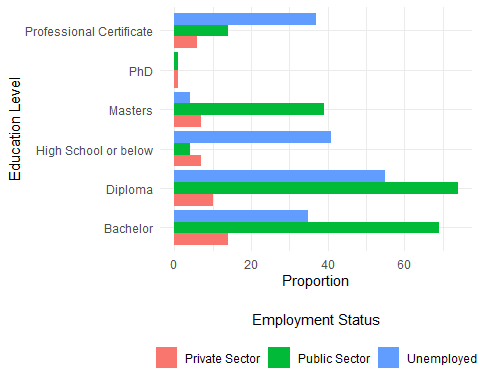
\includegraphics{USAGE_files/figure-latex/unnamed-chunk-16-1.pdf}

\begin{Shaded}
\begin{Highlighting}[]
\CommentTok{\# Calculate the frequency of Piyg and Waye combinations}
\NormalTok{frequency }\OtherTok{\textless{}{-}}\NormalTok{ selected\_columns }\SpecialCharTok{\%\textgreater{}\%}
  \FunctionTok{group\_by}\NormalTok{(Piyg, Waye) }\SpecialCharTok{\%\textgreater{}\%}
  \FunctionTok{tally}\NormalTok{()}

\CommentTok{\# Bar plot}
\NormalTok{bar\_plot }\OtherTok{\textless{}{-}} \FunctionTok{ggplot}\NormalTok{(frequency, }\FunctionTok{aes}\NormalTok{(}\AttributeTok{x =}\NormalTok{ Piyg, }\AttributeTok{y =}\NormalTok{ n, }\AttributeTok{fill =}\NormalTok{ Waye)) }\SpecialCharTok{+}
  \FunctionTok{geom\_bar}\NormalTok{(}\AttributeTok{stat =} \StringTok{"identity"}\NormalTok{, }\AttributeTok{position =} \StringTok{"stack"}\NormalTok{) }\SpecialCharTok{+}
  \FunctionTok{labs}\NormalTok{(}\AttributeTok{title =} \StringTok{"Distribution by Piyg and Waye"}\NormalTok{,}
       \AttributeTok{x =} \StringTok{"Gender"}\NormalTok{,}
       \AttributeTok{y =} \StringTok{"Frequency"}\NormalTok{,}
       \AttributeTok{fill =} \StringTok{"Employment Status"}\NormalTok{)}



\CommentTok{\# Display the plots}
\NormalTok{bar\_plot}
\end{Highlighting}
\end{Shaded}

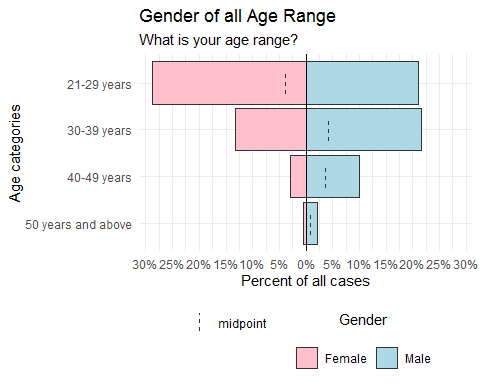
\includegraphics{USAGE_files/figure-latex/unnamed-chunk-17-1.pdf}

\begin{Shaded}
\begin{Highlighting}[]
\FunctionTok{library}\NormalTok{(arsenal)}
\end{Highlighting}
\end{Shaded}

\begin{verbatim}
## 
## Attaching package: 'arsenal'
\end{verbatim}

\begin{verbatim}
## The following object is masked from 'package:lubridate':
## 
##     is.Date
\end{verbatim}

\begin{Shaded}
\begin{Highlighting}[]
\FunctionTok{library}\NormalTok{(kableExtra)}
\end{Highlighting}
\end{Shaded}

\begin{verbatim}
## 
## Attaching package: 'kableExtra'
\end{verbatim}

\begin{verbatim}
## The following object is masked from 'package:srvyr':
## 
##     group_rows
\end{verbatim}

\begin{verbatim}
## The following object is masked from 'package:dplyr':
## 
##     group_rows
\end{verbatim}

\begin{Shaded}
\begin{Highlighting}[]
\NormalTok{table1 }\OtherTok{\textless{}{-}}  \FunctionTok{tableby}\NormalTok{(Iyhwyrts}\SpecialCharTok{\textasciitilde{}}\NormalTok{Piyg }\SpecialCharTok{+}\NormalTok{Hloe}\SpecialCharTok{+}\NormalTok{Waye}\SpecialCharTok{+}\NormalTok{Wiyar, }\AttributeTok{data =}\NormalTok{ USAGE)}
\FunctionTok{summary}\NormalTok{(table1)}
\end{Highlighting}
\end{Shaded}

\begin{longtable}[]{@{}
  >{\raggedright\arraybackslash}p{(\columnwidth - 14\tabcolsep) * \real{0.2966}}
  >{\centering\arraybackslash}p{(\columnwidth - 14\tabcolsep) * \real{0.0966}}
  >{\centering\arraybackslash}p{(\columnwidth - 14\tabcolsep) * \real{0.1172}}
  >{\centering\arraybackslash}p{(\columnwidth - 14\tabcolsep) * \real{0.0828}}
  >{\centering\arraybackslash}p{(\columnwidth - 14\tabcolsep) * \real{0.1310}}
  >{\centering\arraybackslash}p{(\columnwidth - 14\tabcolsep) * \real{0.1172}}
  >{\centering\arraybackslash}p{(\columnwidth - 14\tabcolsep) * \real{0.1034}}
  >{\raggedleft\arraybackslash}p{(\columnwidth - 14\tabcolsep) * \real{0.0552}}@{}}
\toprule()
\begin{minipage}[b]{\linewidth}\raggedright
\end{minipage} & \begin{minipage}[b]{\linewidth}\centering
Good (N=168)
\end{minipage} & \begin{minipage}[b]{\linewidth}\centering
Moderate (N=35)
\end{minipage} & \begin{minipage}[b]{\linewidth}\centering
Poor (N=3)
\end{minipage} & \begin{minipage}[b]{\linewidth}\centering
Very Good (N=156)
\end{minipage} & \begin{minipage}[b]{\linewidth}\centering
Very Poor (N=8)
\end{minipage} & \begin{minipage}[b]{\linewidth}\centering
Total (N=370)
\end{minipage} & \begin{minipage}[b]{\linewidth}\raggedleft
p value
\end{minipage} \\
\midrule()
\endhead
\textbf{Piyg} & & & & & & & 0.422 \\
~~~Female & 81 (48.2\%) & 20 (57.1\%) & 1 (33.3\%) & 64 (41.0\%) & 4
(50.0\%) & 170 (45.9\%) & \\
~~~Male & 87 (51.8\%) & 15 (42.9\%) & 2 (66.7\%) & 92 (59.0\%) & 4
(50.0\%) & 200 (54.1\%) & \\
\textbf{Hloe} & & & & & & & 0.216 \\
~~~N-Miss & 2 & 0 & 0 & 1 & 0 & 3 & \\
~~~Bachelor & 55 (33.1\%) & 10 (28.6\%) & 1 (33.3\%) & 39 (25.2\%) & 0
(0.0\%) & 105 (28.6\%) & \\
~~~Diploma & 54 (32.5\%) & 9 (25.7\%) & 1 (33.3\%) & 52 (33.5\%) & 4
(50.0\%) & 120 (32.7\%) & \\
~~~High School or below & 17 (10.2\%) & 9 (25.7\%) & 0 (0.0\%) & 17
(11.0\%) & 1 (12.5\%) & 44 (12.0\%) & \\
~~~Masters & 16 (9.6\%) & 4 (11.4\%) & 0 (0.0\%) & 27 (17.4\%) & 0
(0.0\%) & 47 (12.8\%) & \\
~~~PhD & 2 (1.2\%) & 0 (0.0\%) & 0 (0.0\%) & 0 (0.0\%) & 0 (0.0\%) & 2
(0.5\%) & \\
~~~Professional Certificate & 22 (13.3\%) & 3 (8.6\%) & 1 (33.3\%) & 20
(12.9\%) & 3 (37.5\%) & 49 (13.4\%) & \\
\textbf{Waye} & & & & & & & 0.030 \\
~~~N-Miss & 1 & 0 & 0 & 2 & 0 & 3 & \\
~~~Private Sector & 22 (13.2\%) & 6 (17.1\%) & 0 (0.0\%) & 9 (5.8\%) & 0
(0.0\%) & 37 (10.1\%) & \\
~~~Public Sector & 80 (47.9\%) & 9 (25.7\%) & 1 (33.3\%) & 85 (55.2\%) &
6 (75.0\%) & 181 (49.3\%) & \\
~~~Unemployed & 65 (38.9\%) & 20 (57.1\%) & 2 (66.7\%) & 60 (39.0\%) & 2
(25.0\%) & 149 (40.6\%) & \\
\textbf{Wiyar} & & & & & & & 0.256 \\
~~~N-Miss & 0 & 0 & 0 & 2 & 0 & 2 & \\
~~~21-29 years & 80 (47.6\%) & 23 (65.7\%) & 2 (66.7\%) & 71 (46.1\%) &
3 (37.5\%) & 179 (48.6\%) & \\
~~~30-39 years & 61 (36.3\%) & 10 (28.6\%) & 0 (0.0\%) & 55 (35.7\%) & 5
(62.5\%) & 131 (35.6\%) & \\
~~~40-49 years & 25 (14.9\%) & 2 (5.7\%) & 1 (33.3\%) & 21 (13.6\%) & 0
(0.0\%) & 49 (13.3\%) & \\
~~~50 years and above & 2 (1.2\%) & 0 (0.0\%) & 0 (0.0\%) & 7 (4.5\%) &
0 (0.0\%) & 9 (2.4\%) & \\
\bottomrule()
\end{longtable}

\hypertarget{likert-scale-analysis}{%
\subsection{Likert Scale Analysis}\label{likert-scale-analysis}}

\begin{enumerate}
\def\labelenumi{\arabic{enumi}.}
\item
  Define latent variables:

  \begin{itemize}
  \item
    Gender: Create a latent variable representing gender, which can be
    indicated by the responses to question 2.
  \item
    Education Level: Create a latent variable representing the highest
    level of education, based on question 3.
  \item
    Employment Status: Create a latent variable representing employment
    status, using the responses from question 4.
  \item
    Age Range: Create a latent variable representing age range, based on
    the responses to question 5.
  \item
    Subscriber Duration: Create a latent variable representing the
    duration of subscription to the National Health Insurance Scheme,
    using the responses from question 6.
  \item
    Access Healthcare: Create a latent variable representing previous
    access to healthcare under the National Health Insurance Scheme,
    based on question 7.
  \item
    Healthcare Delivery: Create a latent variable representing the
    perception of healthcare delivery under the National Health
    Insurance Scheme, using the responses from question 8.
  \item
    Awareness of Mobile Renewal Service: Create a latent variable
    representing awareness of the NHIS Mobile Renewal Service, based on
    the responses to question 9.
  \item
    Mobile Renewal Usage: Create a latent variable representing the
    usage of the Mobile Renewal Service, using the responses from
    question 10.
  \item
    Service Rating: Create a latent variable representing the rating of
    the Mobile Renewal Service, based on the responses to question 11.
  \item
    Service Continuation: Create a latent variable representing the
    agreement on the continuation or suspension of the Mobile Renewal
    Service, using the responses from question 12.
  \item
    Perceived Benefits: Create a latent variable representing the
    perceived benefits of using the Mobile Renewal Service, based on the
    responses to questions 14-17.
  \item
    Usability: Create a latent variable representing the usability of
    the Mobile Renewal Service, using the responses from questions
    18-21.
  \item
    Trust: Create a latent variable representing trust in the Mobile
    Renewal Service, based on the responses to questions 24-27.
  \item
    Accessibility: Create a latent variable representing the
    accessibility of the Mobile Renewal Service, using the responses
    from questions 30-32.
  \item
    Reliability: Create a latent variable representing the reliability
    of the Mobile Renewal Service, based on the responses to questions
    33-34.
  \item
    Data Security: Create a latent variable representing the perception
    of data security in using the Mobile Renewal Service, using the
    responses from questions 35-36.
  \item
    Satisfaction: Create a latent variable representing satisfaction
    with the overall performance of the Mobile Renewal Service, based on
    the responses to question 37.
  \end{itemize}

  \hypertarget{modelling}{%
  \subsection{Modelling}\label{modelling}}
\item
  Define measurement model:

  \begin{itemize}
  \tightlist
  \item
    Assign survey questions to corresponding latent variables as
    indicators. For example, question 2 will be an indicator of the
    Gender latent variable, question 3 will be an indicator of the
    Education Level latent variable, and so on. Assign appropriate
    measurement models (e.g., binary, ordinal, or continuous) based on
    the nature of the survey questions.
  \end{itemize}
\item
  Define structural model:

  \begin{itemize}
  \tightlist
  \item
    Specify the relationships between latent variables based on
    theoretical expectations. For example, we hypothesize that Age
    Range, Gender,Education Level ,Employment Status affects or
    influences awareness of the Mobile Renewal Service.
  \end{itemize}
\item
  Estimate the model:

  \begin{itemize}
  \tightlist
  \item
    Use SEM software (such as lavaan, AMOS, or Mplus) to estimate the
    model parameters. The software will provide estimates for factor
    loadings, regression coefficients, and latent variable variances and
    covariances.
  \end{itemize}

  \hypertarget{model-evaluation}{%
  \subsection{Model Evaluation}\label{model-evaluation}}
\item
  Assess model fit:

  \begin{itemize}
  \tightlist
  \item
    Evaluate the goodness-of-fit of the model using fit indices such as
    the chi-square test, Comparative Fit
  \end{itemize}
\end{enumerate}

\end{document}
